\documentclass{article}

\usepackage{graphicx}
\usepackage{amsmath,amssymb,amsthm} % define this before the line numbering.
\usepackage{color}
\usepackage{eso-pic}
\usepackage{bm}
\usepackage{caption}
%\usepackage{picins}   
\usepackage{microtype}
%\usepackage[mediumspace,mediumqspace,Grey,squaren]{SIunits}
\usepackage{multirow}
\usepackage{epstopdf}
\usepackage{algorithm2e}
\usepackage{url}
\usepackage{enumerate}

% Declaring commonly used math operators
\DeclareMathOperator{\ddiag}{Diag}
\DeclareMathOperator{\rrank}{rank}
\DeclareMathOperator{\vvec}{vec}
\DeclareMathOperator{\tr}{tr}

\newcommand{\PhiB}{\mathbf{\Phi}}
\newcommand{\Ll}{\mathcal{L}}
\newcommand{\Nn}{\mathcal{N}}
\newcommand{\Uu}{\mathcal{U}}
\newcommand{\Ee}{\mathcal{E}}
\newcommand{\Aa}{\mathcal{A}}
\newcommand{\Hh}{\mathcal{H}}
\newcommand{\Ii}{\mathcal{I}}
\newcommand{\Ff}{\mathcal{F}}
\newcommand{\Dd}{\mathcal{D}}
\newcommand{\Tt}{\mathcal{T}}
\newcommand{\Pp}{\mathcal{P}}
\newcommand{\Ss}{\mathcal{S}}
\newcommand{\Cc}{\mathcal{C}}
\newcommand{\Bb}{\mathcal{B}}
\newcommand{\Rr}{\mathcal{R}}
\newcommand{\Rm}{\mathrm{R}}
\newcommand{\CB}{\mathbf{C}}
\newcommand{\RB}{\mathbf{R}}
\newcommand{\xB}{\mathbf{x}}
\newcommand{\yB}{\mathbf{y}}
\newcommand{\ZB}{\mathbf{Z}}
\newcommand{\SB}{\mathbf{S}}
\newcommand{\AB}{\mathbf{A}}
\newcommand{\WB}{\mathbf{W}}
\newcommand{\TB}{\mathbf{T}}

\newcommand{\omitme}[1]{}
\newtheorem*{lemma}{Lemma}
\newtheorem{case}{Case}

\title{Homework 0}

\author{Prateep Mukherjee}

\begin{document}
\maketitle

\noindent 1. (a) 
   
   \begin{itemize}
	\item $A(n) = \Theta \left( 4^{n}\right)$
	 \item $B(n) = \Theta \left( n^{2}\right)$ 
  	 \item $C(n) = \Theta \left( n^{2} \right)$ 
	 \item $D(n) = \Theta \left( n^{log_{3}{2}}\right)$
	 \item $E(n) = \Theta \left( 3^{\frac{n}{2}} \right) $
    \end{itemize}

(b) $ 7^{n}  >> \sqrt{7^{n}} >> 7^{\sqrt{n}} >> 7^{lg(n)} >> 7^{lg(\sqrt{n})} \equiv \sqrt{7^{lg(n)}} >> 7^{\sqrt{lg(n)}} >> lg \: 7^{n} >> lg \: \sqrt{7^n} >> n >> lg \: 7^{\sqrt{n}} >> \sqrt{lg \: 7^n} >> \sqrt{n} >> lg \: n >> lg \: \sqrt{n} > \sqrt{lg \: n}$  \\  

\noindent 2.   (a) List of nodes generated by a preorder traversal are: 

  \begin{itemize}
    \item  Preorder: S Q V I R T Z A P H E B D X F L O G M N Y C K
  \end{itemize}

{\bf Proof:}  S is at the beginning of the inorder traversal and at the last of the post-order traversal. This implies that the left-subtree of S is NULL. Next, V is the immediate neighbor to S in inorder traversal. Hence, this should be the next left child of S. However, it is not directly attached to S. Its father, the node Q, comes immediately after S in post-order traversal. Thus, Q should be the immediate right child of S, and the father of V.

\clearpage
(b) 

 \begin{figure}[!hbt]
    \centering
    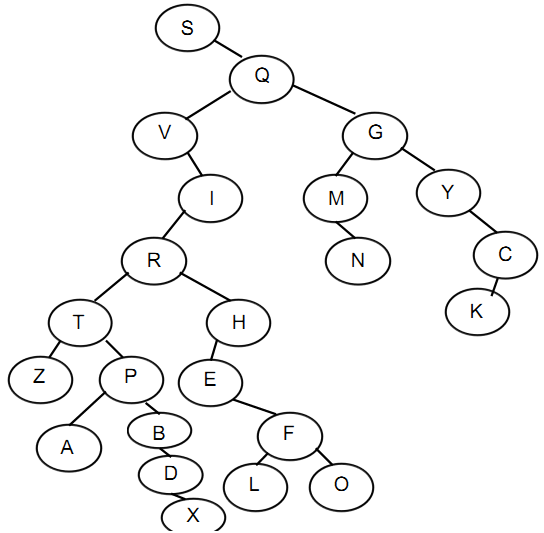
\includegraphics[width=\linewidth]{hw0_2.png}
    \caption{Prof. Giungla's tree}
 \end{figure} 

\clearpage

\noindent 3. A {\em segment-tree} (\url{http://en.wikipedia.org/wiki/Segment_tree}) data-structure can be used to support the given  queries.  A segment-tree is a heap-like structure, where in each node we store the maximum value within a given range in an array. The segment-tree data structure supports two operations: {\em BuildSegmentTree(node,beg,end,T,A,n)} and {\em QuerySegmentTree(node,beg,end,T,A,i,j)}. Here, T is the array storing the segment-tree data-structure. Size of T is O(n), since height of the tree is $\log{n}$ and the maximum number of nodes stored is $2^{lg \: n} \equiv n$. \\
%
%\begin{algorithm}[H]
%	\caption{BuildSegmentTree}
%	   \SetAlgoLined
%	    \KwData{node = 1, b = 1, e = N, T, A, n}
%            \eIf {$ b == e$ } {
%                   $T[node] = b$\;
%	      } {
%                    BuildSegmentTree($2 \times node$, b, $\frac{b+e}{2}$, T, A, n)\;
%		     BuildSegmentTree($2 \times node + 1$, $\frac{b+e}{2} + 1$, e, T, A, n)\;
%		   
%                    \eIf { $A[T[2\times node]]  \leq A[T[2\times node + 1]]$ } {
%                              $T[node] = T[2 \times node + 1]$\;
%		       } {
%                              $ T[node] = T[2 \times node]$ \;
%                     }
%               }
%\end{algorithm}


%\begin{algorithm}[H]
%         \SetAlgoLined
%         \caption{QuerySegmentTree}
%	  \KwData{node, b, e, T, A, i, j}
%	  $ p_{1}, p_{2} : integers $\;
%         \If { $ i > e \: \| \: j < b$ } {
%                   return -1\;
%          } 
%          \If { $ b \geq i \: \& \: e \leq j$ } { 
%                    return T[node]\;
%           }
%
%           $p_1$= QuerySegmentTree($2 \times node$, b, $\frac{b+e}{2}$, T, A, i, j)\;
%           $p_2$ = QuerySegmentTree($2 \times node + 1$, $\frac{b+e}{2} + 1$, e, T, A, i, j)\;
%	    \If { $p_1 == -1$ } {
%                   return $T[node] = p_2$\;
%	     }
%             \If  { $p_2 == -1$ } {
% 			return $T[node] = p_1$\;
%	      }
%             \eIf { $A[p_1] \geq A[p_2]$ } { 
%                      return $T[node] = p_1$\;
%              } {
%                      return $T[node] = p_2$\;
%              }
%\end{algorithm}

\noindent Both the functions above are performed in O($\log{n}$), where n is the number of nodes in the tree. As the preprocessing step, we build two segment-trees, one on $x$-coordinate and the other on $y$-coordinate. The calling function for this operation is $BuildSegmentTree(1, 1, n, T, \Aa, n)$. Lets call these two arrays $T_{x}$ and $T_{y}$ respectively. Having defined the above functions, we can define the functions {\emph HighestToRight}  and {\em RightMostAbove} similarly, as follows.


\begin{figure*}[!h]
\begin{minipage}{2.15in}
	
	\begin{algorithm}[H]
	\caption{HighestToRight(l)}
	   \SetAlgoLined
	   \KwData{point arrays $\Aa$ ($\xB$,$\yB$), l}
	   \KwResult{HighestToRight(l)}
%	   preprocess to generate {\em max-heap} $\Hh$ on y\;
%	   preprocess to generate $\Aa = (x,\Hh(y) )$ \;
%	   BuildSegmentTree(1, 1, n, T, A, n)\;
	   sort $\Aa$ based on $x$-coordinate \;
	   binary-search in $\Aa$ for $i$ s.t. $(x_{i}) \ge l$ \;
	   \If {$\neg \exists{i}$ } {
		return NONE \;
           }	
	    ind = QuerySegmentTree(1, 1, n, $T_x$, A, i, n)\;
           \eIf {$ind == -1$ } {
                 return NONE\;
            } {
                 return $\Aa_{ind} $\;
            }
	\end{algorithm}
\end{minipage}
\hfill
\begin{minipage}{2.15in}
\begin{algorithm}[H]
	\caption{RightmostAbove(l)}
	   \SetAlgoLined
	   \KwData{point arrays $\Aa$ ($\xB$,$\yB$), l}
	   \KwResult{RightmostAbove(l)}
%	   preprocess to generate {\em max-heap} $\Hh$ on y\;
%	   preprocess to generate $\Aa = (x,\Hh(y) )$ \;
%	   BuildSegmentTree(1, 1, n, T, A, n)\;
	   sort $\Aa$ based on $y$-coordinate \;
	   binary-search in $\Aa$ for $i$ s.t. $(y_{i}) \ge l$ \;
	   \If {$\neg \exists{i}$ } {
		return NONE \;
           }	
	    ind = QuerySegmentTree(1, 1, n, $T_y$, A, i, n)\;
           \eIf {$ind == -1$ } {
                 return NONE\;
            } {
                 return $\Aa_{ind} $\;
            }
	\end{algorithm}
\end{minipage}

\end{figure*}

\noindent Size of the segment-tree T is O(n). Building the segment-tree is $O(\log(n))$. Each query is one search in the segment-tree, for both algorithms. So total query time is $O(\log(n))$. \\



\noindent 4.  \begin{lemma}  
  Any arithmetic expression tree can be decomposed into equivalent arithmetic expression tree in normal form.
 \end{lemma}

\noindent {\bf Definitions:}  Let, $E$ denote an expression or non-terminal node and $\Aa$ denote a variable or  terminal node. Therefore, we define the following semantic rules.
            \begin{itemize}
               \item $ E  = E \quad |  \quad E + E \quad | \quad  E \times E \quad |  \quad \Aa$
	      \item $ \Aa = {a , \cdots, z} \quad | \quad \Aa $
             \end{itemize}

Henceforth, we define the leaf nodes of the tree by $\Aa$ and the non-leaf nodes by $E$. Let us also denote 

\begin{proof} We prove the following lemma using the principle of induction.
 
   {\bf [Basis step]} We prove that the lemma is true for $n = 3$.  The diagram given in the figure shows the two possible positions of the operators, $+$ and $\times$. From each of the two positions we can generate an expression tree in normal form.

  {\bf [Inductive step]}  Let us assume the above lemma holds true for $n$ nodes, $\Aa_{1} , \cdots \Aa_{n}$. Let us call this tree $T_n$, which is in normal form. Now, we have to add another term, $\Aa_{n+1}$ to the expression to see if we can generate an expression tree in normal form. The new term $\Aa_{n+1}$ can be appended to  $T_n$ in two ways. (i) $T_n + \Aa_{n+1}$, or (ii) $T_n \times \Aa_{n+1}$. If we append the term $\Aa_{n+1}$ at the front, we can prove our lemma using a similar argument.

\noindent It is evident that an expression tree will not be in its normal form if parent of a +-node is {\bf not} a +-node. That  is, the root of $T_n$ is +-node and we multiply the term $\Aa_{n+1}$ to that, which is shown in the Fig. \ref{fig4}.

\begin{figure}
   \centering
   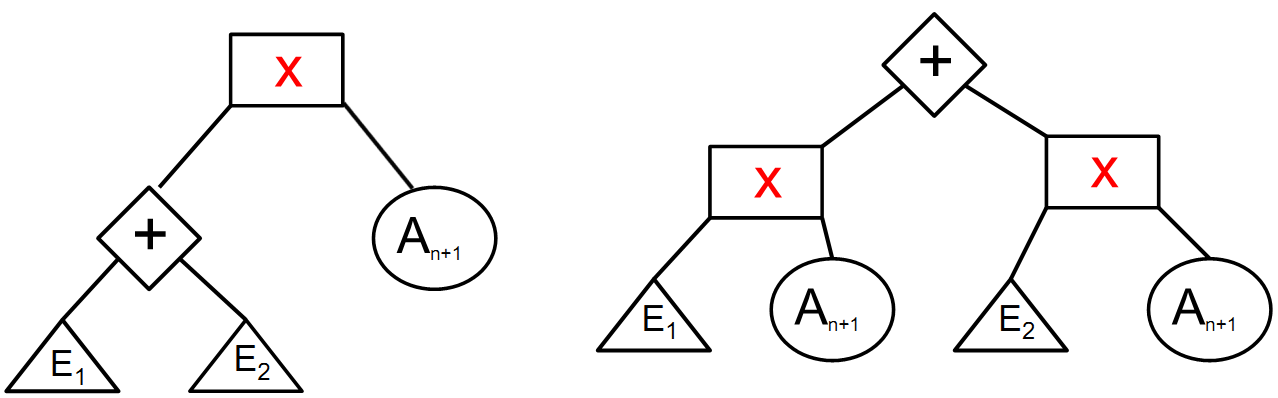
\includegraphics[width=\linewidth]{hw0_4.png}
    \caption{The expression tree(Left) which is transformed to generate the expression tree in normal form(Right).}
    \label{fig4}
\end{figure}

\noindent As seen in Fig. \ref{fig4}, we can transform a given expression tree, not in normal form, to an equivalent expression tree, in normal form, using the above transformation. Also here, the expressions $E_1$ and $E_2$ are in normal form. Hence, the new expression tree $T_{n+1}$ is also in normal form. Hence, proved.

\end{proof}


\noindent 5. (a) The cards are thrown away in a pair. So, each time either 0, or 2, or 4, or 8 etc cards are thrown away. Therefore, 

\vspace{-10pt}

\begin{equation}
    E(\# \: of \: cards \: thrown) = 0 \times P(0) + 2 \times P(2) + \cdots + 102 \times P(102) \notag
\end{equation}

The expected number of cards that are hurled is $\frac{1751}{52}$. \\

(b)  

\begin{enumerate}[i]
  \item $\frac{1}{169}$
  \item $\frac{1}{52}$
  \item $\frac{1}{4}$
  \item $0.0145$
\end{enumerate} 

(c)

\begin{enumerate}[i]
   \item $\frac{1}{13}$
    \item $\frac{17}{52}$
    \item $0$
    \item $\frac{3}{11}$
\end{enumerate}

\end{document}
